% Drawing 154/09-10 -- folder 154, batch 09, archive page 163 (PDF page 164).
% Transcription: un seul dessin en couleur : des courbes vert clair qui se coupent deux à deux, l'une formant une boucle ; les extrémités sont marquées d'un trait bleu, chaque point de croisement porte deux petites flèches noires, et chaque arc entre deux croisements est marqué d'un signe $+$ ou $-$
% Kind: curves crossing pairwise, arcs signed + or -. Method 2 (schematic redraw from the facsimile). Status: ok.
% Notes: Three light green curves are followed on the page (the transcription's note counts four): one that runs from the lower left up over a large loop and leaves at the top, crossing itself once; one from the lower left along the bottom of the loop, turning up on the right and leaving at the top; one from the bottom left straight up to the upper right. Their six ends carry a short blue stroke. Redrawn 2026-11-12 (issue 128): to check again. Question settled by a machine pass on the facsimile, 2026-11-12 (page): three curves, six blue-marked ends. Not checked by a reader. 2026-11-14, Claude Opus 5.5, overlay check (issue 147): rasterised from its own coordinates over the 400 dpi colour scan (402 ppi native) on a unit grid; not compiled (no TeX in the session). Changed: the three curves, read from a page view, lay 1 to 2.5 units off their ink and are retraced on a grid at 10 px per unit (their crossings fall where the traced curves meet); the pairs of small black arrows at the seven crossings, which the transcription names, are added (read at 18 to 25 px per unit), with the small blue blot that sits in the angle of each pair. Signs read again on colour crops: six + (the « + » drawn at (64.4,-23.3) was that blue blot and is removed) and five − (the one between the second crossing and the « + » under it, at (34.2,-44.7), added). Laid over the scan again, every curve, arrow, blot, end stroke and sign lies on its ink to within about 1 unit. Left out: very faint grey curves in the background (an arc under the upper right of the loop, a curve under its lower half), too faint to read and perhaps erased. Status set to ok.
% Coordinates: 1 unit = 1 mm = 1/100 of the crop width (bbox in page fractions: [0.2, 0.085, 0.8, 0.4]).
% Redrawn by Claude (claude-fable-5-2), issue #128, 2026-11-12; not checked by a human; not compiled (no TeX in the session).
% Revised by Claude (claude-fable-5-2) 2026-11-12 (issue #128, triage of the review lines on the 400 dpi colour facsimile): the page has three light green curves: six ends carry a blue stroke (the other small blue marks sit in the angles of crossings), and each curve can be followed from end to end; as drawn. Not checked by a reader; not compiled (no TeX in the session).
% Checked by Claude (claude-opus-5-5) 2026-11-14 (issue #147): overlaid on the 400 dpi colour facsimile; not compiled (no TeX in the session). Not checked by a human. Status: ok.
% Rights: reproduces part of the work -- behind RENDER_TRANSCRIPTS, never published by itself.
\documentclass[tikz,border=3pt]{standalone}
\usepackage{amsmath,amssymb}
\usetikzlibrary{patterns,arrows.meta}
\tikzset{Lg/.style={green!60!black!70}, Bl/.style={blue!70!black}, pencil/.style={black!45}, struck/.style={black!35}, mpt/.style={circle,draw,inner sep=1.3pt}, pt/.style={circle,fill,inner sep=0.9pt}, opt/.style={circle,draw,fill=white,inner sep=1.1pt}}
\begin{document}
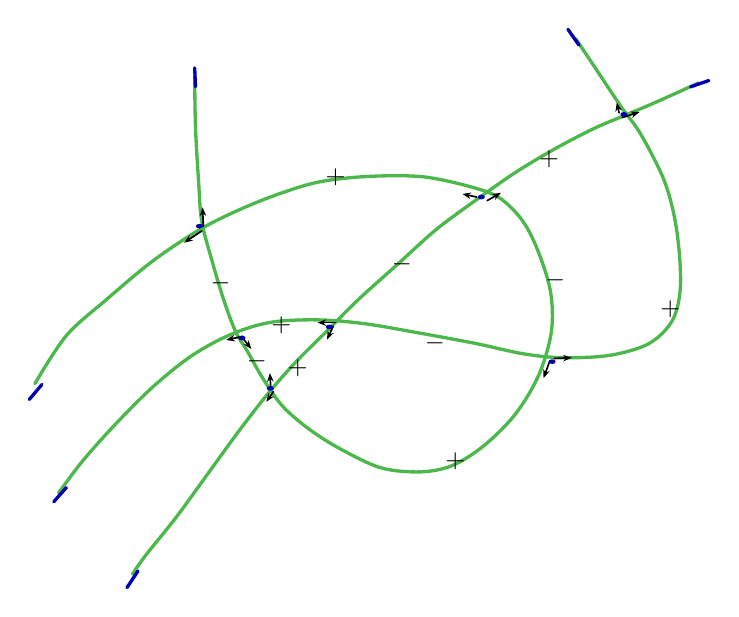
\begin{tikzpicture}[x=1mm,y=1mm,line cap=round,line join=round,font=\scriptsize]
\draw[Lg,very thick] plot[smooth, tension=0.55] coordinates {(6,-47.6) (10,-41.5) (15,-37) (21,-32) (27,-28) (32,-25.5) (37,-23.5) (42,-22) (48,-21.3) (55,-21.3) (61,-22.5) (65,-24) (68,-27) (70,-31) (71.5,-36) (71.6,-41) (70,-46.5) (67,-51.5) (63,-55.5) (59,-58) (55,-58.8) (50,-58.3) (45,-56) (41,-53.5) (37.5,-50.5) (35,-47) (33,-43.5) (31.5,-41) (30,-37) (28.5,-32) (27.2,-27) (26.8,-22) (26.4,-15) (26.3,-8.5)};
\draw[Lg,very thick] plot[smooth, tension=0.55] coordinates {(9,-61.5) (12,-57.5) (16,-53) (21,-48) (26,-44) (31,-41.3) (36,-39.8) (42,-39.5) (48,-40) (55,-41.2) (62,-42.5) (68,-43.8) (73,-44.3) (79,-44) (84,-42.5) (87,-39.5) (88,-35) (87.5,-28) (86,-22) (83,-16) (80.5,-12.5) (77.5,-8) (74.7,-3.8)};
\draw[Lg,very thick] plot[smooth, tension=0.55] coordinates {(18.4,-71.8) (20,-69.5) (24,-64.5) (28,-59) (32,-53.5) (35.5,-49) (39,-45) (43,-41) (47,-37) (52,-32.5) (57,-28) (62,-24.3) (67,-20.8) (72,-17.8) (77,-15.2) (81,-13.5) (85,-11.8) (90.3,-9.4)};
\draw[Bl,very thick] (6.9,-47.7) -- (5.3,-49.6);
\draw[Bl,very thick] (26.4,-9.9) -- (26.3,-7.5);
\draw[Bl,very thick] (10,-60.8) -- (8.4,-62.6);
\draw[Bl,very thick] (75.1,-4.6) -- (73.7,-2.6);
\draw[Bl,very thick] (19.1,-71.4) -- (17.7,-73.5);
\draw[Bl,very thick] (89.3,-9.9) -- (91.6,-9.1);
\node[inner sep=1pt] at (44.2,-21.4) {\small $+$};
\node[inner sep=1pt] at (71.3,-19.1) {\small $+$};
\node[inner sep=1pt] at (86.7,-38.2) {\small $+$};
\node[inner sep=1pt] at (37.3,-40.2) {\small $+$};
\node[inner sep=1pt] at (39.4,-45.6) {\small $+$};
\node[inner sep=1pt] at (59.4,-57.5) {\small $+$};
\node[inner sep=1pt] at (29.6,-34.8) {\small $-$};
\node[inner sep=1pt] at (52.6,-32.5) {\small $-$};
\node[inner sep=1pt] at (72.1,-34.5) {\small $-$};
\node[inner sep=1pt] at (56.8,-42.5) {\small $-$};
\draw[semithick,-{Stealth[length=1.1mm]}] (27.4,-27.6) -- (27.3,-25.2);
\draw[semithick,-{Stealth[length=1.1mm]}] (27.2,-28.2) -- (24.95,-29.7);
\draw[semithick,-{Stealth[length=1.1mm]}] (62.1,-23.9) -- (60.3,-23.5);
\draw[semithick,-{Stealth[length=1.1mm]}] (63.45,-24.35) -- (65.2,-23.35);
\draw[semithick,-{Stealth[length=1.1mm]}] (32.4,-41.6) -- (30.3,-42.05);
\draw[semithick,-{Stealth[length=1.1mm]}] (32.5,-41.95) -- (33.5,-43.2);
\draw[semithick,-{Stealth[length=1.1mm]}] (44.2,-39.85) -- (41.9,-39.85);
\draw[semithick,-{Stealth[length=1.1mm]}] (43.9,-40.3) -- (43.1,-42);
\draw[semithick,-{Stealth[length=1.1mm]}] (35.95,-48) -- (35.85,-46.25);
\draw[semithick,-{Stealth[length=1.1mm]}] (36.3,-48.6) -- (35.4,-49.9);
\draw[semithick,-{Stealth[length=1.1mm]}] (72,-44.4) -- (74.2,-44.3);
\draw[semithick,-{Stealth[length=1.1mm]}] (71.4,-44.7) -- (70.6,-46.9);
\draw[semithick,-{Stealth[length=1.1mm]}] (80.2,-13.2) -- (79.9,-11.9);
\draw[semithick,-{Stealth[length=1.1mm]}] (80.6,-13.8) -- (82.8,-13.1);
\node[inner sep=1pt] at (34.2,-44.7) {\small $-$};
\fill[Bl] (26.9,-27.6) ellipse[x radius=0.45, y radius=0.3];
\fill[Bl] (62.7,-23.9) ellipse[x radius=0.45, y radius=0.3];
\fill[Bl] (32.3,-41.8) ellipse[x radius=0.45, y radius=0.3];
\fill[Bl] (43.4,-40.4) ellipse[x radius=0.45, y radius=0.3];
\fill[Bl] (35.9,-48.2) ellipse[x radius=0.45, y radius=0.3];
\fill[Bl] (71.7,-44.8) ellipse[x radius=0.45, y radius=0.3];
\fill[Bl] (80.8,-13.4) ellipse[x radius=0.45, y radius=0.3];
\end{tikzpicture}
\end{document}
